\documentclass[a4paper,12pt]{book}
\usepackage[utf8]{inputenc}
\usepackage[T1]{fontenc}
\usepackage[frenchb]{babel}
\usepackage{a4wide}
\usepackage{graphicx}
\graphicspath{{images/}}
\usepackage{subfig}
\usepackage{tikz}
\usetikzlibrary{shapes,arrows}
\usepackage{pgfplots}
\pgfplotsset{compat=newest}
\pgfplotsset{plot coordinates/math parser=false}
\newlength\figureheight
\newlength\figurewidth
\pgfkeys{/pgf/number format/.cd,
set decimal separator={,\!},
1000 sep={\,},
}
\usepackage{ifthen}
\usepackage{ifpdf}
\ifpdf
\usepackage[pdftex]{hyperref}
\else
\usepackage{hyperref}
\fi
\usepackage{color}
\hypersetup{
colorlinks=true,
linkcolor=black,
citecolor=black,
urlcolor=black}

\renewcommand{\baselinestretch}{1.05}
\usepackage{fancyhdr}
\pagestyle{fancy}
\fancyfoot{}
\fancyhead[LE,RO]{\bfseries\thepage}
\fancyhead[RE]{\bfseries\nouppercase{\leftmark}}
\fancyhead[LO]{\bfseries\nouppercase{\rightmark}}
\setlength{\headheight}{15pt}

\let\headruleORIG\headrule
\renewcommand{\headrule}{\color{black} \headruleORIG}
\renewcommand{\headrulewidth}{1.0pt}
\usepackage{colortbl}
\arrayrulecolor{black}

\fancypagestyle{plain}{
  \fancyhead{}
  \fancyfoot[C]{\thepage}
  \renewcommand{\headrulewidth}{0pt}
}

\makeatletter
\def\@textbottom{\vskip \z@ \@plus 1pt}
\let\@texttop\relax
\makeatother

\makeatletter
\def\cleardoublepage{\clearpage\if@twoside \ifodd\c@page\else%
  \hbox{}
  \thispagestyle{empty}
  
  \if@twocolumn\hbox{}\newpage\fi\fi\fi}
\makeatother

\usepackage{amsthm}
\usepackage{amssymb,amsmath,bbm}
\usepackage{array}
\usepackage{bm}
\usepackage{multirow}
\usepackage[footnote]{acronym}

\parskip=5pt

\begin{document}

% Première page
\begin{titlepage}
\begin{center}


\includegraphics[width=0.6\textwidth]{logo_univ2}\\[1cm]

{\large Licence 2 Informatique - HLIN405}\\[0.5cm]

{\large Projet tutoré}\\[0.5cm]

% Titre
\rule{\linewidth}{0.5mm} \\[0.4cm]
{ \huge \bfseries Hashiwokakero \\[0.4cm] }
\rule{\linewidth}{0.5mm} \\[1.5cm]

% Auteurs et encadrant
\noindent
\begin{minipage}{0.4\textwidth}
  \begin{flushleft} \large
    \emph{Auteurs :} \\
    M. Thomas \textsc{Di Giovanni} \\
    M. Thomas \textsc{Bertin} \\
  \end{flushleft}
\end{minipage}
\begin{minipage}{0.4\textwidth}
  \begin{flushright} \large
    \emph{Encadrant :} \\
    M.~Philippe \textsc{Janssen} \\
  \end{flushright}
\end{minipage}

\vfill

% Bas de la page
{\large Version 0.1 du \\ \today}

\end{center}
\end{titlepage}

% Table des matières
\tableofcontents
\clearpage

% Contenu du rapport
\mainmatter
\pagestyle{fancy}

\cleardoublepage

\chapter*{Introduction}
\addcontentsline{toc}{chapter}{Introduction}
\markboth{Introduction}{Introduction}
\label{chap:introduction}

Cette année, nous avons eu pour tâche de nous rassembler par groupe afin d'effectuer un projet TER tout au long du second semestre. Dans le cadre de ce dernier, nous avons eu l'opportunité d'avoir un enseignant et/ou chercheur nous encadrant. Celui-ci nous aidait alors chaque semaine lors de réunions sur certains points du projet, nous permettant, la plupart du temps, de nous débloquer et de nous aider à nous avancer sur la suite du projet en nous répartissant au mieux les tâches. \newline
Notre travail était donc porté sur un casse-tête appelé "Hashiwokakero" ou plus simplement "Hashi". Ainsi nous avons eu pour but de créer son résolveur afin de le résoudre le plus efficacement possible à l'aide de nos connaissances en algorithmique et en programmation C++. \newline
Concernant le déroulement du projet, nous avons choisi de concentrer notre programme sur GitHub. Ce choix a eu deux différentes raisons de naître, la première concernait l'utilisation de Git qui nous permettait alors de synchroniser le travail effectué à la fin de chaque session de programmation et la deuxième concernait le côté pratique puisque nous pouvons ainsi partager le travail entre nous, étudiants et encadrant, afin que ce dernier puisse voir notre avancement et que nous puissions voir celui de l'autre. \newline
De ce fait, tout cela nous a mené à créer notre projet et son rapport dont voici le plan. \newline
Tout d'abord, nous allons aborder les domaines de l'informatique dans lequel se situe notre projet en les présentant. Puis nous nous attarderons sur le problème précis sur lequel nous avons travaillé. Ensuite, nous assisterons à la description détaillée et expliquée de notre travail. Et pour finir, nous achèverons sur une conclusion faisant part de nos perspectives ouvertes par notre projet ainsi que l'avenir du programme. Nous pouvons aussi trouver à la toute fin de ce rapport, des remerciements ainsi que la bibliographie regroupant les ouvrages sur lesquels nous nous sommes appuyés.
\chapter{Domaines de l'informatique concernés}
\label{chap:domaines}

Notre projet relève de plusieurs domaines informatiques.
\newline
Premièrement, l'algorithmique. En effet, l'algorithmique est l'étude et la production d'un ensemble de règles opératoires, présent dans ce qu'on appelle un algorithme, dont l'application permet de résoudre un problème énoncé au moyen d'un nombre fini d'opérations. Ainsi, avant de commencer la programmation, nous avons réfléchi à des algorithmes permettant de nous aider à savoir comment le programmer mais aussi d'avoir une meilleure idée de comment notre code fonctionnera. C'est à ce moment-là que nous avons réfléchi à comment modéliser les données de notre problème. Au tout début, nous avons donc réfléchi en jouant au casse-tête s'il existait un moyen d'optimiser notre façon de résoudre le Hashi afin d'être plus rapide et dans le but de réaliser le meilleur temps entre nous. Ainsi, nous avons commencé par écrire, au brouillon, des algorithmes contenant des conditions et des boucles de manière à trouver ce qu'on appellera plus tard des règles qui nous permettent de détecter les cas les plus triviaux et, à partir de là, d'élucider le reste du casse-tête de façon plus simple. 
\smallbreak
Deuxièmement, la programmation objet, car c'est avec le langage C++ que nous avons décidé de travailler, et c'est avec des objets que nous représentons ces données. Ce langage va nous permettre de pouvoir modéliser notre problème et donc de pouvoir y travailler concrètement dessus (Figure 1.1). Le langage C++ nous étant imposé, nous n'avons pas eu à avoir le choix parmi les autres langages objets existant, cependant, ceci ne nous dérangeait absolument pas du fait que nous préférions ce langage à d'autres langages qui nous étaient moins connus. En effet, parmi les centaines de langages de programmation qui existent, certains sont plus populaires que d'autres. Sans aucun doute, le C++ est un langage très populaire et c'est principalement pour cela que nous l'avons à apprendre au cours de notre cursus. La popularité n'est pas le seul critère de ce dernier puisque c'est en effet un langage puissant et particulièrement rapide le rendant essentiel pour le développement de jeux par exemple. Ainsi, pour résumer grossièrement, nous pouvons dire qu'il est très répandu, aidant ainsi la compréhension de ce dernier puisque nous pouvons obtenir de l'aide plus aisément, qu'il est rapide, utilisé pour des applications qui ont besoin de performances et qu'il est portable sur toutes les plates-formes telles que Windows, Mac OS et Linux.\newline

\begin{figure}[htp]
  \centering
  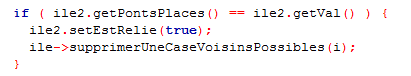
\includegraphics[width=13cm]{images/exemplec++}
  \caption{Exemple de code en C++}
\end{figure}

\chapter{Problème travaillé}
\label{chap:probleme}

Notre but, pour cette UE, était de créer un résolveur fonctionnel de n'importe quelle instance de notre casse-tête. Le nôtre, le Hashiwokakero, consiste à trouver comment relier des îles entre elles à l'aide de ponts. Le jeu se présente donc sous la forme d'une grille d'îles non reliées (Figure 2.1). 
\newline
\begin{figure}[htp]
  \centering
  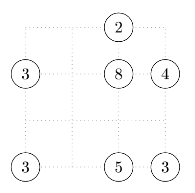
\includegraphics[width=4cm]{images/GrilleHashi}
  \caption{Grille Hashi avant résolution}
\end{figure}

Afin de résoudre une instance et de trouver une solution au problème qui se pose dans le Hashi, il faut que toutes les îles soient reliées par un nombre de ponts égal au degré de l'île concernée (degré qui sera compris entre 1 et 8, car il est impossible de placer plus), mais aussi que toute île soit accessible à partir de n'importe quelle autre île, autrement dit que le réseau soit connexe. Il ne peut cependant n'y avoir qu'un maximum de deux ponts directs entre deux îles, et ces ponts là ont pour obligation d'être soit verticaux, soit horizontaux. De même, les ponts ne peuvent pas se croiser, ou encore traverser une île et celles-ci ne peuvent être collées côte à côte. Nous noterons aussi qu'il n'existe qu'une seule et unique solution à chaque instance. (Figure 2.2) 
\newline \newline 

\begin{figure}[htp]
  \centering
  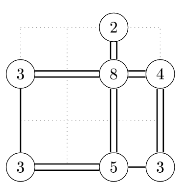
\includegraphics[width=4cm]{images/GrilleHashiResolu}
  \caption{Grille Hashi après l'application de l'unique résolution}
\end{figure}

Pour réaliser cela, nous avons dû:
\begin{itemize}
    \item définir des types de données pour représenter les données de notre problème
    \item réfléchir aux structures de données pour la résolution du casse-tête
    \item écrire des algorithmes de résolution et les programmer
    \item expérimenter les différentes méthodes
    \item faire une trace graphique de la résolution
\end{itemize}

\smallbreak
Trouver une solution à ce problème est NP-complet. NP-complet signifie que c'est un problème non-déterministe, c'est-à-dire, que nous ne pourrons pas résoudre ce casse-tête de façon polynomiale sur toutes les possibilités qu'il existe. De plus, il se peut que nous ne trouvions pas la solution du premier coup, et donc que nous soyons obligés de retenter la résolution en prenant le problème différemment. 
\smallbreak
Avant d'entrer plus en détail dans notre façon de traiter le problème, nous allons définir quelques notions. Premièrement, nous appellerons un pont simple un pont reliant les mêmes îles. De la même façon, un double pont correspond à deux ponts reliants les même îles.
\newline
Ensuite, une île sera considérée comme "résolue" lorsque son degré sera égal à son nombre de ponts. La grille du casse-tête sera elle considérée comme résolue lorsque la solution au problème sera trouvée.
\newline
Enfin, une île est considérée comme voisin possible d'une autre île si les deux peuvent être directement reliées, tandis qu'une île est considérée comme voisin réel d'une autre île si les deux sont déjà reliées. Il est important de noter cependant que dans cette façon de voir les choses, une île peut être à la fois voisin possible et réel d'une autre île (e.g. une île reliée par un pont simple sera considérée comme un voisin réel, mais restera dans les voisins possibles si elle n'est toujours pas résolue).
On appellera valeur restante d'une île, le nombre de ponts placés de l'île soustrait à son degré. Autrement dit, le nombre de ponts qu'il est encore possible de placer.
\smallbreak
Afin de trouver comment relier les îles correctement, nous avons établi des "règles" pour la création de pont: Notre première règle consiste à dire qu'une île ayant une valeur restante égale au double de son nombre de voisins possible aura un pont double entre elle et chacun de ses voisins possibles. En effet cela est le seul moyen pour l'île d'être résolue et nous permet donc de saturer ces îles là, nous ouvrant alors d'autres éventuelles possibilités sur le reste de la grille. (Figure 2.3 et 2.4)\newline

\begin{figure}[htp]
  \centering
  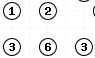
\includegraphics[width=3cm]{images/Regle1}
  \caption{Îles avant l'application de la règle 1}
\end{figure}

\begin{figure}[htp]
  \centering
  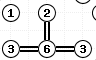
\includegraphics[width=3cm]{images/Regle1_2}
  \caption{Îles après l'application de la règle 1}
\end{figure}


Notre seconde règle consiste à dire que si la valeur restante d'une île plus un correspond au double du nombre de voisins possibles de cette même île, alors un pont simple peut être placé sur tous ses voisins possibles Dans le cas particulier où l'île et un de ses voisins possibles sont déjà reliés par un pont simple, on passe le pont simple en pont double. Cependant, cette règle ne fonctionne que sur les îles ayant un degré impair. (Figure 2.5 et 2.6)
\newline
Si à la suite de cette deuxième règle la valeur restante de l'île correspond à son nombre exact de voisins possibles, alors on "remplit" l'île, c'est à dire que nous plaçons un deuxième pont entre l'île concernée et tous ses voisins possibles, créant ainsi des ponts doubles. En effet, il se peut que le nombre de voisins possibles de l'île ait pu changer suite à la règle, et ce dans le bon sens, c'est-à-dire, de façon à ce que les deux valeurs précédents soient égales permettant alors le remplissage de l'île par des doubles ponts puisque nous rappelons que cette "règle" ne se produit qu'après l'application de la deuxième et donc qu'il y a déjà des ponts simples placés. (Figure 2.7) \newline

\begin{figure}[htp]
  \centering
  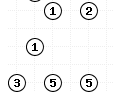
\includegraphics[width=3.5cm]{images/Regle2_1}
  \caption{Îles avant l'application de la règle 2}
\end{figure}

\begin{figure}[htp]
  \centering
  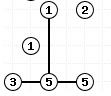
\includegraphics[width=3.5cm]{images/Regle2_2}
  \caption{Îles après l'application de la règle 2}
\end{figure}

\begin{figure}[htp]
  \centering
  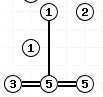
\includegraphics[width=3.5cm]{images/Regle2_3}
  \caption{Suite de la règle 2 - Cas particulier}
\end{figure}
\chapter{Description du travail réalisé}
\label{chap:description}

Pour réaliser ce projet, nous avons décidé de créer plusieurs structures de données afin de représenter le problème et de le résoudre, représentées par des classes dans le langage C++.

\section{Donnée "Ile"}
Notre structure de donnée Ile contient plusieurs informations:
\begin{itemize}
    \item son degré
    \item sa coordonnée en abscisse dans la grille
    \item sa coordonnée en ordonnée dans la grille
    \item le nombre de ponts reliés à cette île
    \item un tableau d'îles qui représente les voisins possibles
    \item un tableau d'îles représentant les voisins réels
    \item un booléen qui sera vrai si l'île est résolue, faux sinon
\end{itemize}
\smallbreak
Pour finir, nous avons aussi ajouté deux attributs à notre structure Ile concernant les composantes connexes. Nous avons décidé de les représenter comme des arbres: on désigne une île comme étant "chef" de sa composante connexe, et toutes les autres îles de cette composante seront "fils" (directs ou non, cependant il est préférable qu'ils soient directs pour la suite) de celui-ci. Les deux attributs à ce sujet sont donc la hauteur de l'arbre représentant la composante connexe à laquelle l'île appartient, ainsi qu'un pointeur vers une autre île de la composante connexe qui sera son père direct dans l'arbre.
\smallbreak
En ce qui concerne les méthodes de cette classe, la grande majorité ne changera que l'île concernée (accesseurs) et une seule interagit avec un autre objet: DéjàVoisin. Son but est de vérifier si l'île dans laquelle est appelée la méthode est déjà reliée à celle passée en paramètre (autrement dit si elle fait partie des voisins réels). Cette méthode renvoie un booléen.

\section{Donnée "Pont"}
Notre structure de donnée Pont ne contient que peu d'informations:
\begin{itemize}
    \item un pointeur vers la première île
    \item un pointeur vers la deuxième île
    \item le "nombre" de ponts (simple ou double)
    \item un booléen vrai si le pont est vertical, faux sinon
\end{itemize}
\smallbreak
Concernant le nombre de ponts, celui-ci sera égal à un s'il n'existe qu'un seul pont entre les deux îles, ou égal à deux s'il en existe deux. Dans notre vision des choses, deux ponts entre les mêmes îles sera considéré comme un seul objet Pont avec son attribut "nombre" ègal à deux plutôt que deux objets Pont distincts l'un de l'autre.

\section{Donnée "IleOuPont"}
Après avoir créé deux structures de donnée, Ile et Pont, nous avons fait le choix d'en créer une regroupant, en quelque sorte, ces deux dernières. En effet, les deux seuls attributs présents dans IleOuPont sont deux informations concernant le fait de savoir s'il s'agit d'une île ou bien d'un pont, comme nous aurions pu le deviner au vu du nom de cette dernière. Par conséquent, il existe dans cette classe, un attribut se trouvant être un pointeur de Ile et un attribut se trouvant être un pointeur de Pont. De plus, elle contient, en plus des attributs précédemment cités :
\begin{itemize}
    \item Trois constructeurs de classe différents afin de déclarer un objet de ce type de plusieurs manières avec notamment le constructeur par défaut, le constructeur où l'on passe en paramètre un pointeur de type Ile et le constructeur où l'on passe en paramètre un pointeur de type Pont.
    \item Deux accesseurs en écriture afin d'opérer directement un changement sur une ile ou sur un pont.
    \item Deux accesseurs en lecture afin pouvoir récupérer l'île ou le pont présent 
\end{itemize}
\smallbreak
Cette structure de donnée fut créée dans un but précis qui était celui de vouloir créer un vecteur à deux dimensions des îles ou des ponts présents dans la grille. Ainsi chaque case, représentée par des coordonnées en abscisse et en ordonnée, comportait une donnée de type IleOuPont. Afin de savoir s'il s'agissait d'une île ou d'un pont, cette dernière, comme expliqué précédemment, comporte deux attributs servant à le déterminer. S'il s'avérait être un pont alors le pointeur sur Ile serait NULL et inversement ce serait le pointeur sur Pont qui serait NULL. Nous pouvons très bien aussi n'avoir ni de pont ni d'île dans cette case auquel cas les deux attributs seraient NULL mais dans tous les cas, nous ne pouvons avoir les deux attributs non NULL en même temps.

\section{Donnée "Grille"}
Dans cette dernière partie de ce chapitre, nous allons aborder un point important qui est celui de la classe Grille. Elle ne comporte pas moins de sept attributs la complétant :
\begin{itemize}
    \item Un entier signé représentant la hauteur max de la grille de jeu
    \item Un entier signé représentant la longueur max de la grille de jeu
    \item Le vecteur à deux dimensions des îles ou des ponts dans la grille précédemment évoqué
    \item Un booléen signalant si toutes les îles sont résolues
    \item Un entier représentant le nombre de composantes connexes 
    \item Un entier représentant le nombre d'îles présentes
    \item Un entier représentant le nombre d'îles devenues résolues
\end{itemize}
\smallbreak
Tout d'abord il est bon de savoir , avant de commencer quelconque approfondissement, que nous introduisons un fichier texte lors de la compilation de notre programme contenant des informations essentielles sur la grille de jeu. En effet, ce dernier contient notamment la hauteur max et la longueur max de la grille présents dans les attributs de notre classe. Ainsi, nous récupérons ces données à l'aide d'une des méthodes présentes dans Grille, la méthode "lecture", qui elle même va en appeler d'autres afin de procéder à la construction de la grille à partir du fichier texte. Cette méthode va, dans un premier temps, récupérer la hauteur et la longueur max pour ensuite y initialiser la grille et pour finir en y rajoutant les îles dans celle-ci. Effectivement, nous pouvons aussi trouver dans le fichier texte les coordonnées en abscisse et en ordonnée de chacune des îles présentes ainsi que leur valeur, permettant ainsi leur placement. \newline
Ensuite, c'est aussi dans cette classe que nous allons trouver la méthode d'affichage. Cette dernière nous permet donc d'avoir un aperçu concret de notre jeu avec les différentes îles représentées par leur valeur reliées par des ponts simples ou doubles, verticaux ou horizontaux symbolisés par des traits tels que "--", "==", "|" ou encore "||". \newline
De surcroît, nous avons bien évidemment, différents accesseurs en lecture et en écriture concernant tous nos attributs précédemment cités. Plus précisément, nous pouvons par exemple, grâce à "getUneIleOuUnPont", accéder à ce que contient une case précise dans le vecteur à deux dimensions à l'aide de coordonnées. De même pour "setUneIleOuUnPont" où il s'agit, ici, de remplir une case par une île ou un pont de la classe IleOuPont.  \newline
Concernant la notion de composante connexe présente dans la classe Grille, nous nous assurons simplement de savoir combien de composante connexes reste-il afin de déterminer si nous pouvons considérer la grille comme résolu. Pour ce faire, nous vérifions si nous obtenons qu'une seule composante connexe et nous vérifions aussi si toutes les îles sont résolues, et si c'est le cas, alors la grille l'est aussi. Quand à la méthode "unionComposantesConnexes" prenant deux pointeurs de Ile en paramètre, elle a pour but d'unifier les deux composantes connexes de ces îles, qui sont reliées entre elles par un pont, en leur inscrivant, ce qu'on a appelé, le même chef qui n'est autre qu'une île père de toutes les autres îles dans sa composante. \newline
Pour finir, nous avons aussi écrit des méthodes ayant trait aux voisins des îles avec notamment "RecupVoisinsPossibles" nous permettant de récupérer les voisins de notre île sur lesquels il est possible d'y relier au moins un pont. Cette dernière est complétée, en quelque sorte, par "majVoisinsReels" qui va être appelée lorsque nous allons créer un pont afin d'effectuer une mise à jour de tous les voisins de toutes les îles. De ce fait, nous avons trois méthodes principales liées entre elles, "tracerPont" qui va appeler "reglesPonts" lorsque nous tombons sur une île dans la grille. Ensuite, "reglesPonts" va vérifier les règles précédemment expliquées et va donc appeler (notamment) "creerPont" lorsque nous entrerons dans une de ces règles. Et pour terminer, "creerPont" déterminera la nature du pont afin que celui-ci puisse être affiché et effectuera donc la mise à jour des voisins réels. Ces dernières méthodes sont essentielles quand au fonctionnement de notre résolveur.





\section{Fichier "Main"}
Lorsque l'on appelle notre résolveur dans un terminal, un fichier texte doit être passé en paramètre dans lequel est inscrit la taille de la grille (sa largeur et sa hauteur), ainsi que toutes les îles sous la forme "x y degré". Une fois appelé, le résolveur va, dans le main, extraire du fichier les informations avec les méthodes prévues à cet effet. Ensuite, nous ferons une première traversée entière de la grille afin d'initialiser les voisins possibles de toutes les îles (méthode RecupVoisinsPossibles). Nous continuons en faisant appel à la méthode tracerPonts de grille. Une fois la grille résolue, on affiche dans le terminal la solution trouvée. \newline

\begin{figure}[htp]
  \centering
  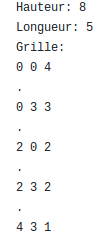
\includegraphics[width=2.35cm]{images/FichierTexte}
  \caption{Fichier texte passé en paramètre}
\end{figure}

\chapter*{Conclusion et remerciements}
\addcontentsline{toc}{chapter}{Conclusion et remerciements}
\markboth{Conclusion}{Conclusion}
\label{chap:conclusion}

Ce projet nous a tout d'abord permis d'appliquer nos connaissances sur un problème concret et ainsi d' enrichir notre expérience. En effet, le fait de réaliser un projet de cette envergure nous a servi à nous tester sur nos compétences en programmation. Nous avions eu, d'ores et déjà au premier semestre, un défi de ce genre avec le jeu TenTen. Seulement, celui-ci, ne proposait pas la réflexion que nous a posé le Hashi puisqu'il s'agissait simplement d'un jeu et non d'un casse-tête. C'est pourquoi, avoir eu l'opportunité de travailler sur des projets comme celui-ci a pu améliorer notre expérience général, que ce soit en terme de programmation mais aussi de réflexion.\newline
Il nous a aussi entraîné à améliorer la gestion de notre temps, qui n'a pas toujours été optimale. Effectivement, afin de produire dans les temps un projet, il nous faut de l'organisation. Ce type "d'épreuve" permet ainsi de se prendre en main en nous faisant réaliser l'ampleur de ce qu'il y a faire. Cela nous aide à être encore plus autonome dans notre travail mais, pour autant, cela nous aide aussi à apprendre à travailler en groupe. Ces dernières notions sont d'autant plus importantes lorsqu'il s'agira de réaliser la demande de notre employeur ou de notre client quand nous trouverons un boulot après nos études. Ainsi, nous pouvons dire que ce type de projet est très important pour nous afin d'être au plus prêt lorsque cela arrivera.
\smallbreak
Malgré tout, notre programme n'est pas complet et ne permet pas de résoudre les problèmes les plus complexes, qui sont les cas où plus aucune de nos règles ne peuvent être appliquées. En effet, dans certaines configurations de départ, il se peut qu'aucune règle ne puisse être mis en oeuvre. Dans ce cas là, il faut alors commencer par essayer différentes combinaisons de ponts entre les îles de manière aléatoire et ainsi débloquer la situation, entraînant l'activation d'une des règles. Néanmoins, il est possible que la façon de commencer ne soit pas la bonne et mène à nulle part. Il faut alors repartir de zéro et, à nouveau, recommencer d'une autre manière jusqu'à trouver l'unique et bonne solution.\newline
Nous n'avons pas aussi eu le temps de s'attarder sur les règles concernant la connexité. Effectivement, il en existe et servent éventuellement à débloquer certaines situations ou du moins à les compléter. Dans notre version du Hashi, nous nous sommes penchés sur la connexité finale, c'est-à-dire, si nous avons bien qu'une seule composante connexe à la fin mais nous n'avons créé aucune règle similaire à celles existantes les concernant. Or il s'avère qu'elles peuvent permettre la création de ponts. Malgré cela, ces dernières ne sont pas indispensables, du moins, elles n'apparaissent que dans de rares cas.
\smallbreak
Pour finir, nous tenons particulièrement à remercier notre encadrant M. Philippe Janssen qui a su nous aider tout au long du projet grâce aux réunions hebdomadaires et notamment à l'aide de ses remarques sur notre travail mais aussi à l'aide de ses remarques sur notre organisation de travail. Cette aide nous a permis de nous débloquer à maintes reprises et nous a permis de savoir quoi faire lors de certaines situations.\newline


\appendix
\nocite{*}
\bibliographystyle{authoryear-fr}
\bibliography{references}

\clearpage

\end{document}